\begin{frame}{What is a cloud?}
	\begin{center}
		\begin{figure}
			\centering
			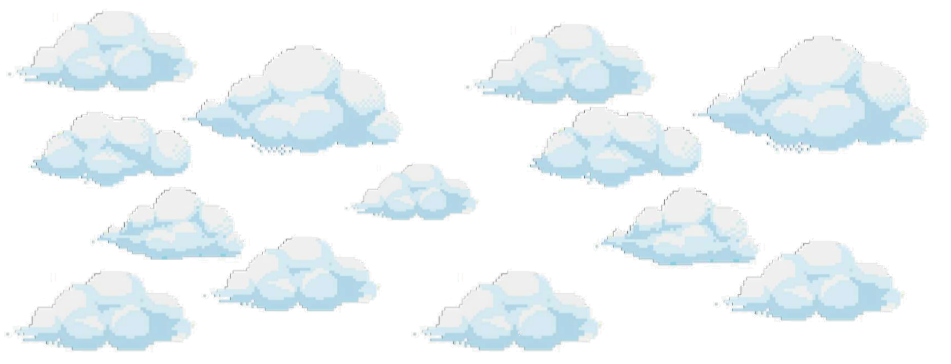
\includegraphics[width=0.8\linewidth]{images/intro_fig00_0.png}
			\label{fig:introfig01}
	\end{figure}
	\vspace{20px}
	\textbf{A cloud is a mass of water drops or ice crystals suspended in the atmosphere.}	
	\end{center}
\end{frame}


\begin{frame}{What is a cloud?}
	\begin{center}
		\begin{figure}
			\centering
			\includegraphics[width=0.7\linewidth]{images/cloud_types.pdf}
			\label{fig:introfig01}
		\end{figure}
		\textbf{A cloud is a mass of water drops or ice crystals suspended in the atmosphere.}	
	\end{center}
\end{frame}

\begin{frame}{What is a cloud?}
	\begin{center}
		\begin{figure}
			\centering
			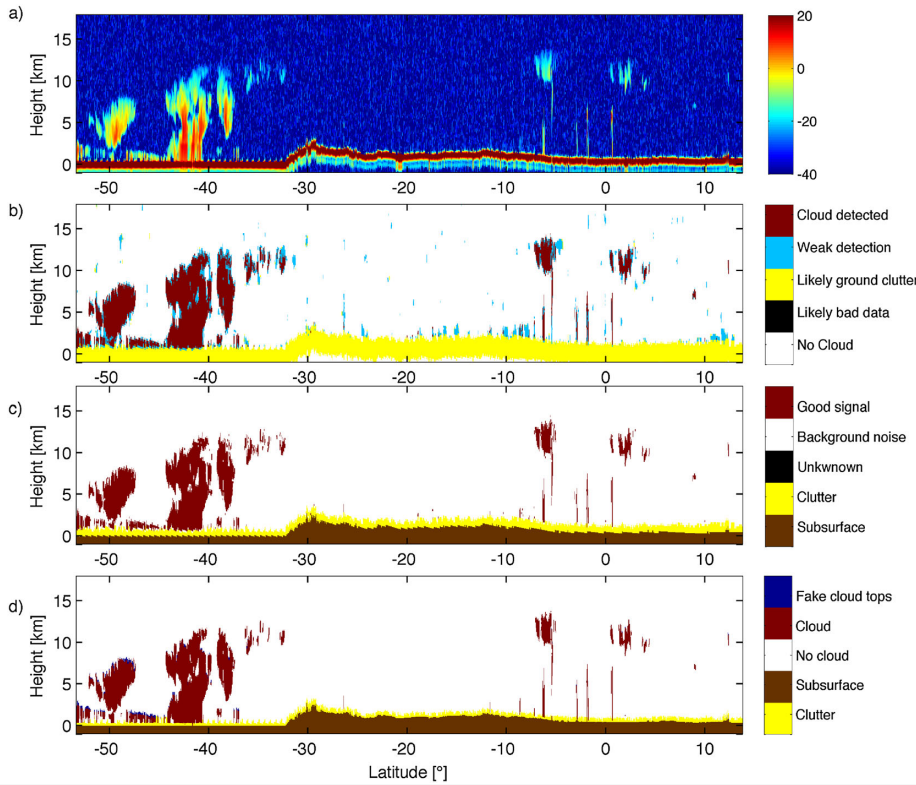
\includegraphics[width=0.65\linewidth]{images/cloud_types2.png}
			\label{fig:introfig01}
		\end{figure}
		\textbf{Cloud classification - CloudSat (Ceccaldi, et al. 2020)}	
	\end{center}
\end{frame}

\begin{frame}{How do cloud cover algorithms work?}
	\begin{center}
		\begin{figure}
			\centering
			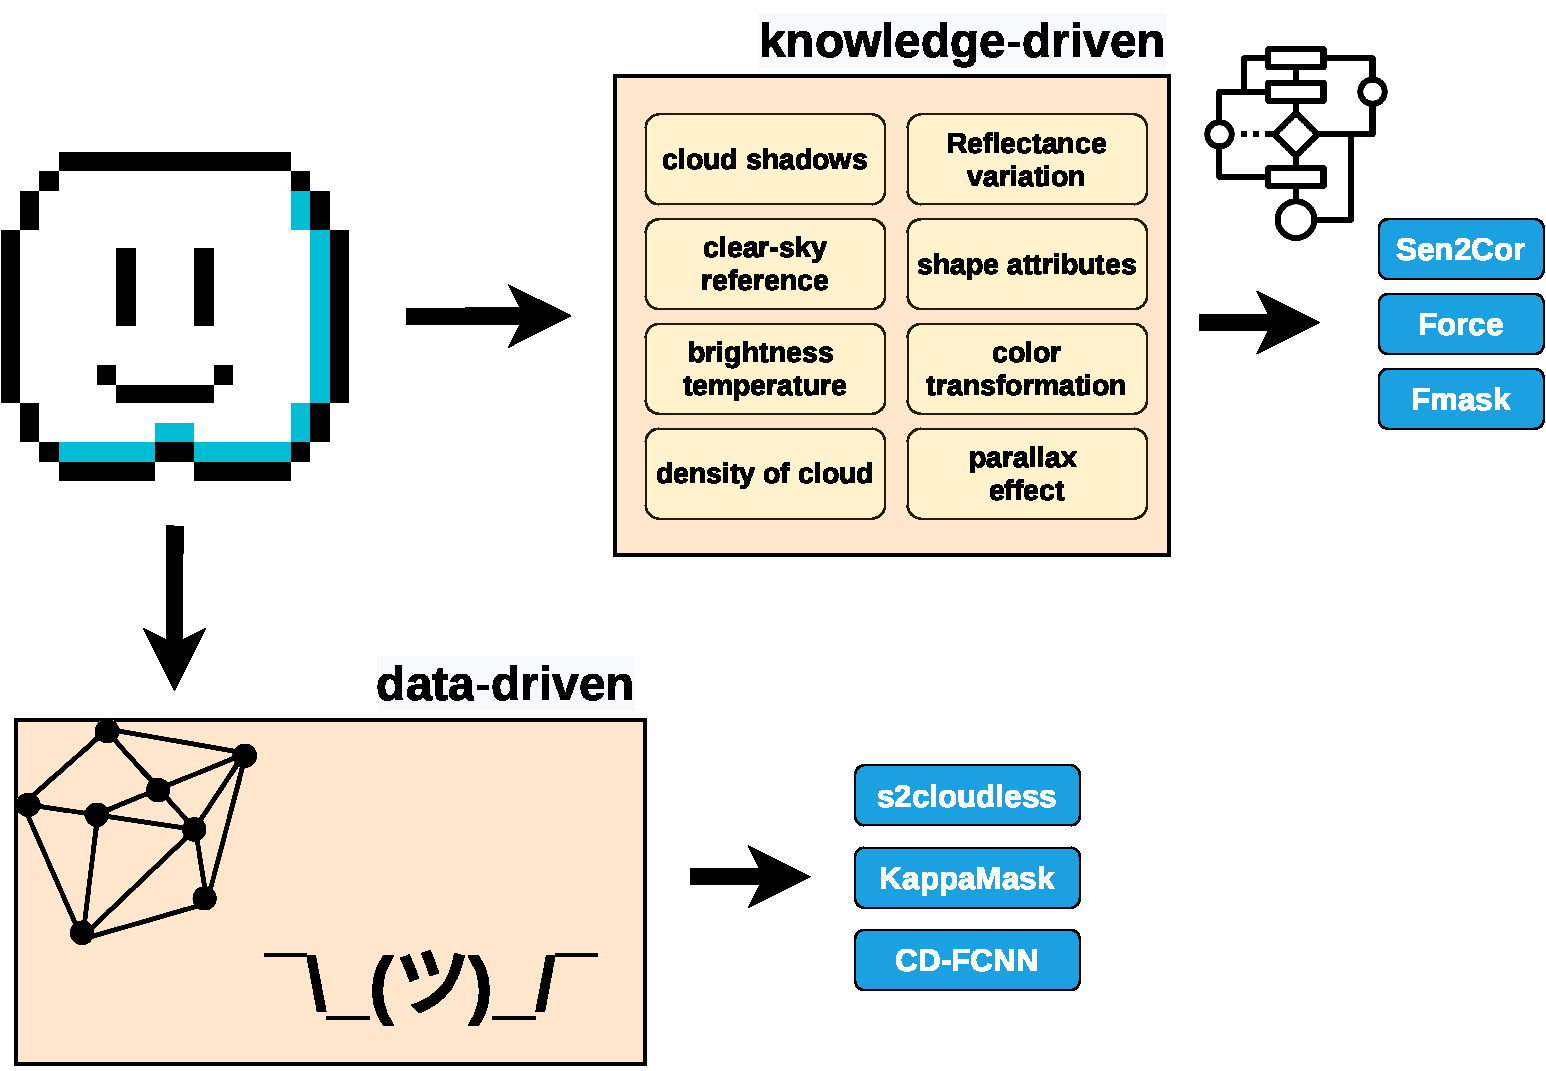
\includegraphics[width=0.85\linewidth]{images/intro_what_is_a_cloud.pdf}
			\label{fig:introfig01}
		\end{figure}
	\end{center}
\end{frame}


\begin{frame}{Context}
	\begin{center}
		\begin{figure}
			\centering
			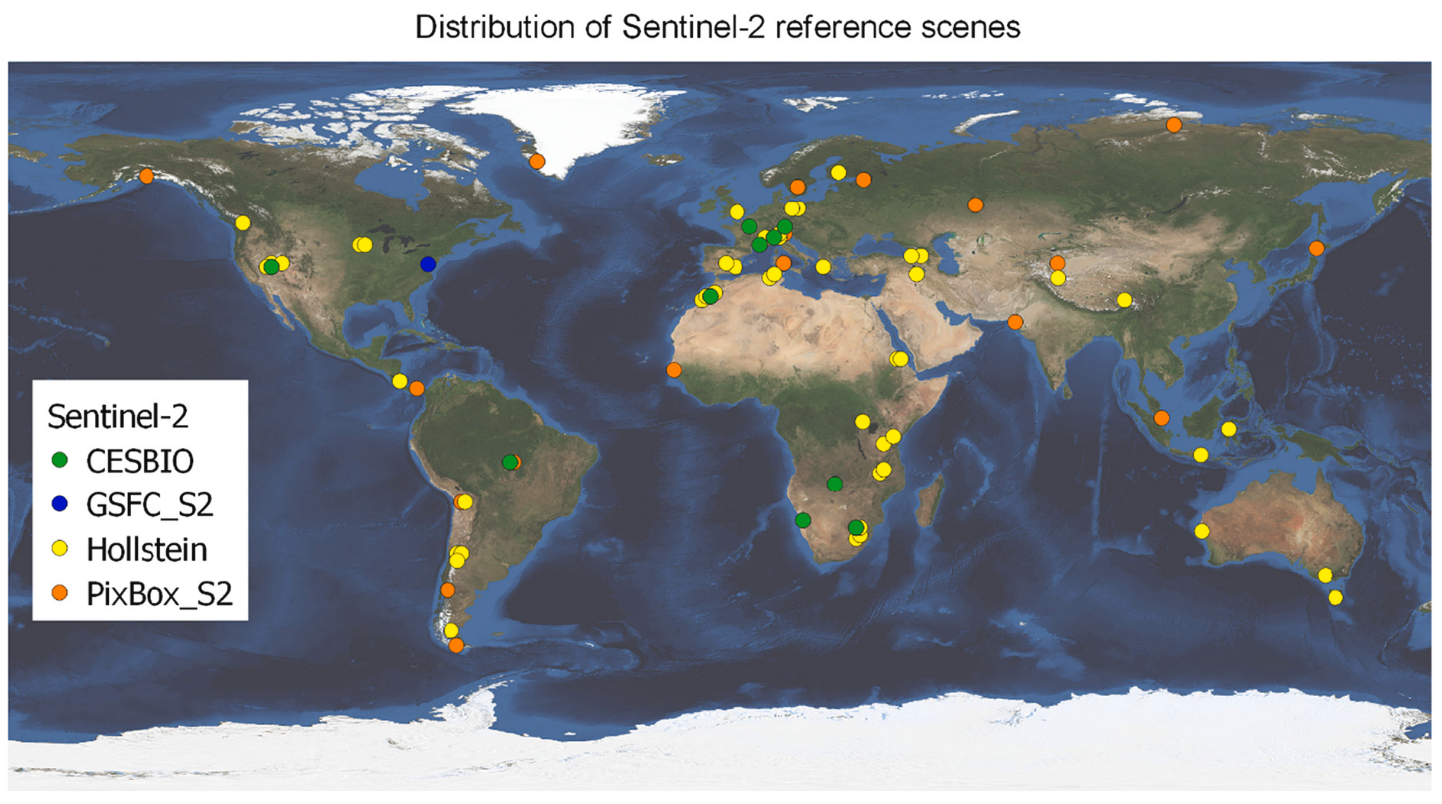
\includegraphics[width=0.85\linewidth]{images/intro_fig01.png}
			\caption[fig:introfig01]{Geographical distribution reference cloud detection datasets for Sentinel-2 (Skakun et al. 2022).}
			\label{fig:introfig01}
		\end{figure}
	\end{center}
\end{frame}
